\subsection{Update of the development plan}

As we tried to remain consistent between reports, we see that the development plan doesn't have to change that much.
The way we split the different modules didn't change, neither did the estimated time allocated to each.
Therefore, we send you back there for the Gantt diagram.
The only restriction we'll have is about the validation with the ID card.
As said in section \ref{SEC:valid_ID} the implementation might be quite tricky, so we weren't able to estimate precisely how much time it would need to implement this.
We planned on implementing this along with the \textit{validation} module, but it might take more time.\\

However, we still had to allocate each module to each other.
Here's what we decided :
\begin{itemize}
  \item \textbf{Core Dev}:
  \begin{itemize}
    \item Database: Julien et Benjamin
    \item Model: Matthieu et Benoit
    \item Display: Alex et Ludovic
  \end{itemize}
  \item \textbf{Modules X}:
  \begin{itemize}
    \item Connection/Subscribing system: Vincent et Pierre-Yves
    \item Validation: Alex et Benoit
    \item Account manager: Vincent et Pierre-Yves
    \item Group manager: Alex et Vincent
    \item Organisations: Benjamin et Ludovic
    \item Offer/Demand creator: Julien et Benoit
    \item Search system: Matthieu et Julien
    \item Transaction acknowledgement: Benjamin et Ludovic
  \end{itemize}
\end{itemize}

\subsection{Design Pattern}

In this section we present one additional design patterns that seems relevant.\\

Most other design patterns are present implicitly in the UML and ORM.
However, one thing that we didn't present in details previously is about the complete structure of a user.\\
Indeed, in our architectural report, we only stated that a user has some mandatory informations and a profile, without going into more details about this profile. The profile is used to contain all the informations a user can inform about himself, like his city, his hobby's,... These informations are not mandatory as they do not determinate the identity (and uncity) of the user, but are important though, because that's what will be used for some service features (e.g. for the advanced search, for the profile page, for the social part of the platform). This allowed us to be more flexible about what a profile will contain. Indeed, we have to be able to add some fields in the future if we think they are relevant.\\

The use of a design pattern also allows us to change it later without changing the entire structure of the class diagram. The chosen pattern design is Facade\footnote{\url{http://www.go4expert.com/articles/design-pattern-simple-examples-t5127/\#facade}}.\\
We will present below some of the profile features we thought to be important right now, but we will have to keep in mind that the profile must be extensible during implementation.

\begin{figure}[H]
  \centering
  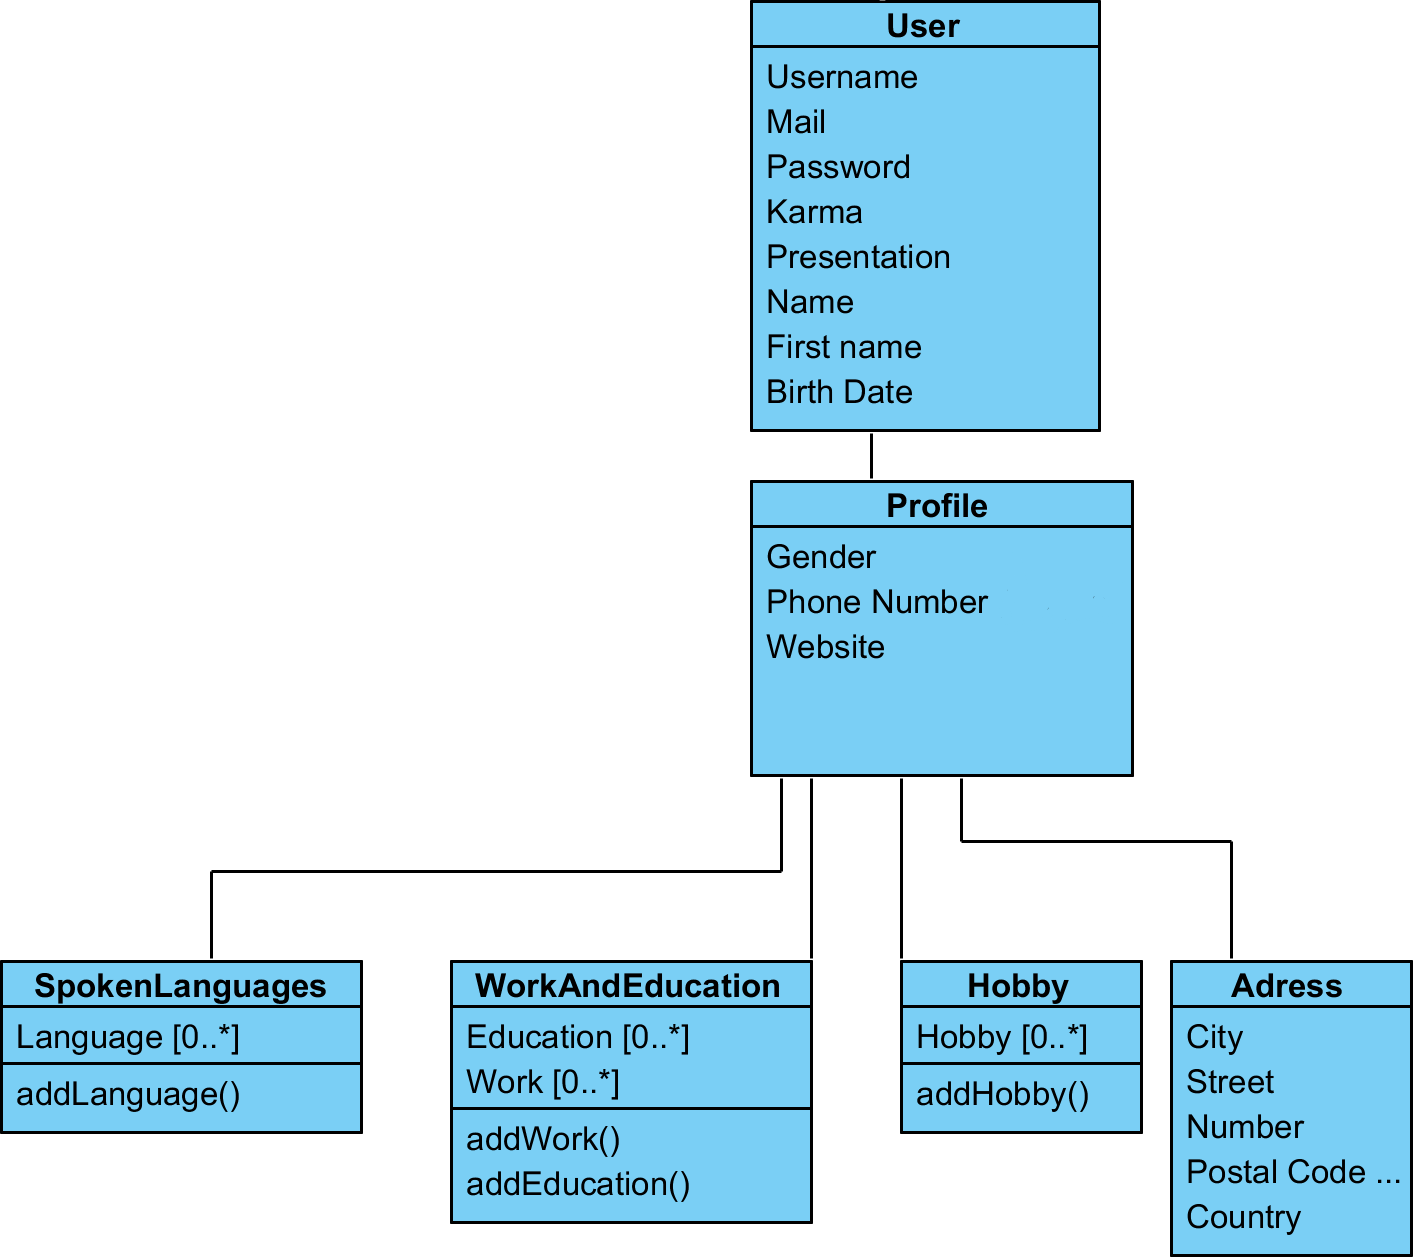
\includegraphics[width=0.5\textwidth]{userprofile.png}
  \caption{User with Profile}
  \label{fig:UserProfile}
\end{figure}

In the figure \vref{fig:UserProfile}, only the information related to a user's profile are represented, for informations related to the user's state (verified, id checked,...) see the class diagram \vref{fig:uml}.

\subsection{Coding Conventions}
\label{SEC:conventions}
With Ruby on Rails, coding conventions are a key feature of good programming. Indeed, as stated in the course's notes and beforehand in the official site's homepage, favouring conventions over configuration is one the main goal of RoR.\\
Therefore we decided to gather all the good conventions practices for RoR to make our application more easy to read and understand, and in order to remain consistent over all our work (no matter which one of us designed a particular feature).\\

Most of the conventions are designed to improve the readability of the code. Today's computer allows us not to worry so much about tiny performance optimisation that makes basically no difference. In essence, the code must be always as easy as possible to understand.\\

To do so, we will first use simple RoR conventions:
\begin{itemize}
	\item The most basics ones are using blank space between methods' arguments, using two spaces instead of tabs, write line shorter than 80 characters (100 at most), etc.
    \item Concerning names, class names will be formatted with camel case (e.g. \texttt{ClassName}) whereas almost all other names (variables, routing,...) will be formatted with snake case (e.g. \texttt{variable\_name}). The only exception is for constants which will be written as in many other languages, with upper case (e.g. \texttt{CONSTANT\_NAME}). All the names should be intuitive and meaningful.
    \item Concerning controller methods, they should be as small as possible (most of the time a few lines are enough), long controller methods usually mean that something is not designed well and may mean it's necessary to re-think the implementation of a feature.
	\item Of course, since we are in a MVC model, views should not touch databases.
\end{itemize}

In addition to that, Rails provide some syntactic sugar or idioms to make the code more readable. For example, it is possible to avoid easily using \texttt{not} in conditional: instead of using \texttt{if not}, we should use the \texttt{unless} keyword, and instead of \texttt{while not}, the \texttt{until} keyword. Another good practice is for iterations, when a particular structure provide an iterating feature, we should use it via the \texttt{each} keyword, e.g.:\\
\indent\texttt{colors.each do |color| \textit{some instructions} end}\\ instead of:\\
\indent\texttt{for color in colors}\\

For comments, we will be careful to not use too many of them. According to some programmers, in an extreme way, no comment should be needed at all, the code being so easy to read that it doesn't need any additional explanation.\\
In practice, we do not aim for such goal but we will try to use them smartly:
\begin{itemize}
	\item First of all, we will try to limit ourselves in using them.
	\item Then, we will delete old comments that are deprecated.
	\item A good use is to favourite comments for a method or even an entire class, explicating the overall goal of the method (class), rather than small comments inside the code as they are very likely to be deprecated fast as the implementation evolves.
	\item Comments will also be used in a \textit{how to way} meaning they will rather explain how to use the commented method or class rather than explaining how it works.
\end{itemize}
This will force us to write simple code.\\

Finally, concerning Git\footnote{Git is a distributed revision control and source code management (SCM) system}, we will use meaningful commit message. Also, if a modification requires many commits\footnote{A commit is a set of changes, a new \textit{revision}} (e.g.: adding a feature), we will work on a separated branch to be able to filter commits more easily.\\

Concerning comments, an addition to the previous paragraph is that if we modify some lines of code and if we want to keep the old version (for safety), we won't leave the code commented, we can simply delete it as it is saved in the revision control system. This is possible very simply (for example to find back that peace of code) if the commit's messages are eloquent.

\subsection{Programming heuristic}

In this section, we will briefly describe the way we are going to work for the implementation phase.

Concerning the tools we are going to use to help us during the implementation, there are many things we can consider: a revision control software, a scheduling tool.\\
As revision control software, we chose to use Git in addition with a repository at Github. Git meets most of our requirements, and with that it will be easy to browse amongst the different revisions, plus the different branches. As explained in section \vref{SEC:conventions}, we will rely a lot on branches. Moreover, Git is the recommended version control system to use with Ruby on Rails.\\
We are planning on the strong use of tests during the implementation (mostly, unit tests, not to be confused with the simulator). This is why we chose Github, which can be linked to Travis, a Continuous Integration (CI) system, to perform automatic build and tests.\\

As a way of working, we will split work in different parts as explained in the last report, which will allows us to work independently. To communicate over each other's progress, we will use Trello, a web-based project management application, to easily see what has been done, what is yet to do and by who, and what is being done right now.\\

As much as possible, we will split the work in teams of two to be able to do pair programming which can be very efficient to avoid errors and to share ideas.\\
Finally, regular meeting will allow to discuss more important matter (like big implemtation choices) and clarify the state of the implementation.